\documentclass[12pt, a4paper]{article}

\usepackage{graphicx}
\usepackage{float}
\usepackage{hyperref}

\hypersetup{
	colorlinks=true,
	linkcolor=black
}


\begin{document}
	\pagenumbering{gobble}
	\begin{titlepage}
		\makebox[\textwidth]{\large  Department of Electrical and Electronic Engineering}
		\vspace*{1.5cm}
		\makebox[\textwidth]{\large University of Johannesburg}
		\makebox[\textwidth]{\textbf{EEP3B21 2018}}
		\vspace*{1.5cm}
		\makebox[\textwidth]{\textit{Lecturer: Dr. AR Ndjiongue}}
		\makebox[\textwidth][l]{\large ELECTRONICS}
		\vspace*{1.5cm}
		\makebox[\textwidth][r]{\large Group Project}
		\vspace*{0.5cm}
		\makebox[\textwidth]{\LARGE Group Project 2 Report}
		\vspace*{0.1cm}
		\makebox[\textwidth]{\large Ruan de Bruyn - 216054484}
		\vspace*{0.1cm}
		\makebox[\textwidth]{\large Quintin Kruger - 216054484}
		\vspace*{0.1cm}
		\makebox[\textwidth]{\large Wesley Richardson - 216054484}
		\vspace*{0.3cm}
		\makebox[\textwidth]{\today}
		\vfill
		\noindent I hereby declare that, except where specifically indicated, the work submitted herein is my own original work\\
		Signed: \hspace*{5cm} Date:
	\end{titlepage}

	\pagenumbering{roman}
	\tableofcontents
	\newpage
	\pagenumbering{arabic}

\section{Theoretical Background}
\label{sec:theoretical_background}
	\subsection{Modulator}
		Amplitude modulation is the simplest modulation technique. A high frequency signal is modulated to carry a lower frequency signal (the lower frequency signal cannot be transmitted effectively as the antenna required to receive a signal with a low frequency is required to be long in length - he length of the antenna is inversely proportional to the frequency it is to receive). The high frequency signal is known as the carrier signal while the signal that needs to be transmitted is called the message signal.

		To implement a modulator circuit, consider the 3 components that need to be made up by the circuit:
		\begin{enumerate}
			\item Carrier frequency generator
			\item Message frequency generator
			\item AM modulator
		\end{enumerate}

		The modulator circuit used for this experiment is shown in the figure below

		\begin{figure}[H]
			\centering
			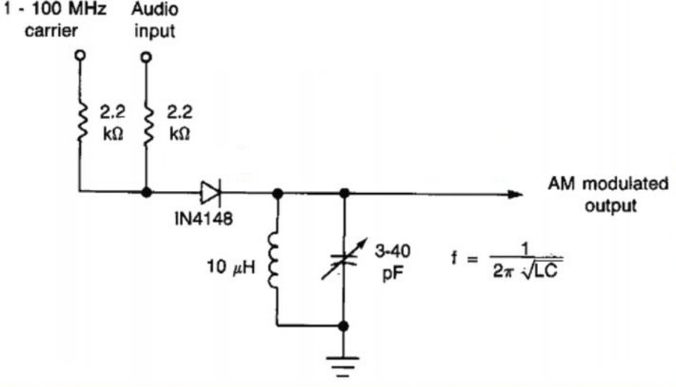
\includegraphics[width=0.7\textwidth]{images/modulator_circuit.png}
			\label{fig:modulator_circuit}
			\caption{The circuit used to implement the modulator.}
		\end{figure}

		The figure shows a frequency equation given as $\frac{1}{2\pi\sqrt{LC}}$. This equation is used to find the value of the capacitor for the modulator circuit (as shown in Figure \ref{fig:modulator_circuit}).
	\subsection{Demodulator Circuit}

		A demodulator circuit is one of the applications of a diode as a detector for amplitude modulated (AM) radio signals. An AM signal consists of a radio-frequency carrier wave whose amplitude varies with different audio frequencies. The detector circuit is essentially a half-wave rectifier circuit with an RC filter placed on the output as can be seen from the circuit of the modulator circuit for this practical in Figure \ref{fig:demodulator_circuit}. The RC time constant of the filter should fall between 2 values

		\begin{equation}
			\label{eqn:time_const_demodulator_circuit}
			\frac{1}{\omega_c} \le RC \le \frac{\sqrt{1-\mu^2}}{\omega_m\mu}
		\end{equation}

		where $\omega_c$ is the frequency of the carrier, $\omega_m$ is the angular frequency of the information and $\mu$ is the modulation index. This result comes from practical experience in the field of electronic engineering rather than from a mathematical principles. If the $RC$ time constant is too small, there would be ripples of the carrier frequency on the output (this is to be avoided as we require the information sent rather than the distortion thereof with the carrier signal). If the $RC$ time constant is too big, it will significantly attenuate high frequencies.


		\begin{figure}[H]
			\centering
			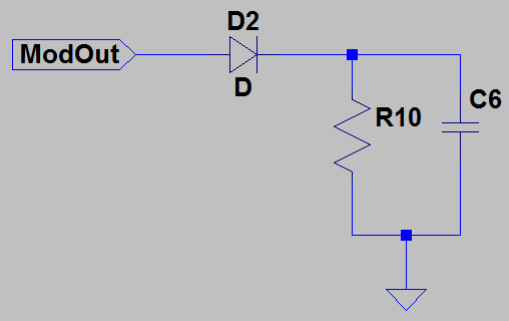
\includegraphics[width=0.7\textwidth]{images/Demodulator_circuit.png}
			\caption{The demodulator circuit used for this experiment}
			\label{fig:demodulator_circuit}
		\end{figure}

	\subsection{Amplifier Circuit} % (fold)
	\label{sub:amplifier_circuit}
	 An amplifier circuit will be used to amplify the demodulated signal which is the output of the demodulator circuit (as discussed in the previous section). 2 requirements are needed to amplify a signal.
	 \begin{enumerate}
	 	\item Gain
	 	\item Filtering
	 \end{enumerate}

	 A gain will give the desired amplification needed while the filter filters out noise from the signal received before it is sent to the amplifier.

	 A common-emitter configuration of the transistor is desired in this practical as it provides us with a high voltage gain. 

	 Consider the circuit given in Figure \ref{fig:transistor_configuration_circuit} which shows the transistor configuration to be used in this experiment.


	 \begin{figure}
	 	\centering
		\label{fig:transistor_configuration_circuit}
		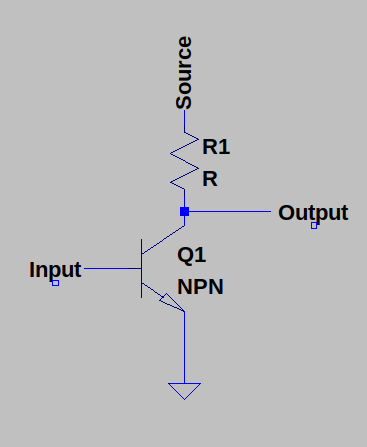
\includegraphics[width=0.7\textwidth]{images/transistor_configuration_circuit.png}
		\caption{Transistor configuration to be used for this experiment}
	 \end{figure}

 	The voltage at the collector terminal of the circuit has to be half that of the source voltage, thus $V_C = \frac{1}{2}V_{CC}$ where $V_{CC}$ is the source voltage.

 	Using ohms law, the collector resistor $R_1$ (as shown in Figure \ref{fig:transistor_configuration_circuit}) can be calculated
 	\begin{equation}
 		R_c = R_1 = \frac{V_{CC}-V_C}{I_C}
 	\end{equation}

 	Where the collector current $I_C$ is current through the collector. The collector current is transistor specified and is calculated using the data sheet provided for the transistor in question. 

 	The voltage gain of the circuit is given as $G = \frac{R_1}{R_e}$ where $R_e$ is the internal resistance of the transistor and is once again transistor specific. The value of $R_e$ is calculated from the equation given as 

 	\begin{equation}
 		R_e = \frac{0.026}{I_e}
 	\end{equation}

 	and is based on the assumption that the collector and the emitter currents are approximately the same.

 	The internal resistance of a transistor is highly unstable (that is its resistance value changes based on changes in the temperature of the material), to account for this instability in the internal resistance of the transistor an additional resistance needs to be included in the transistor circuit. The gain is then given as 

 	\begin{equation}
 		G = \frac{R_1}{R_2 + R_e}
 	\end{equation} 

 	The circuit that incorporates the second resistor is shown in Figure \ref{fig:transistor_configuration_circuit_added_R2}

 	\begin{figure}
 		\centering
		\label{fig:transistor_configuration_circuit_added_R2}
		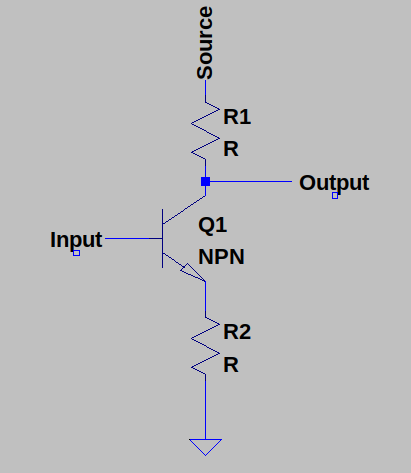
\includegraphics[width=0.7\textwidth]{images/transistor_configuration_circuit_added_R2.png}
		\caption{Changed transistor circuit that accounts for fluctuating R_e}
 	\end{figure}
	% subsection amplifier_circuit (end)



\section{Experimental Method} % (fold)
\label{sec:experimental_method}
	The circuit constructed for this experiment is shown in Figure \ref{fig:circuit_1}
	\begin{figure}[H]
		\centering
		\label{fig:circuit_1}
		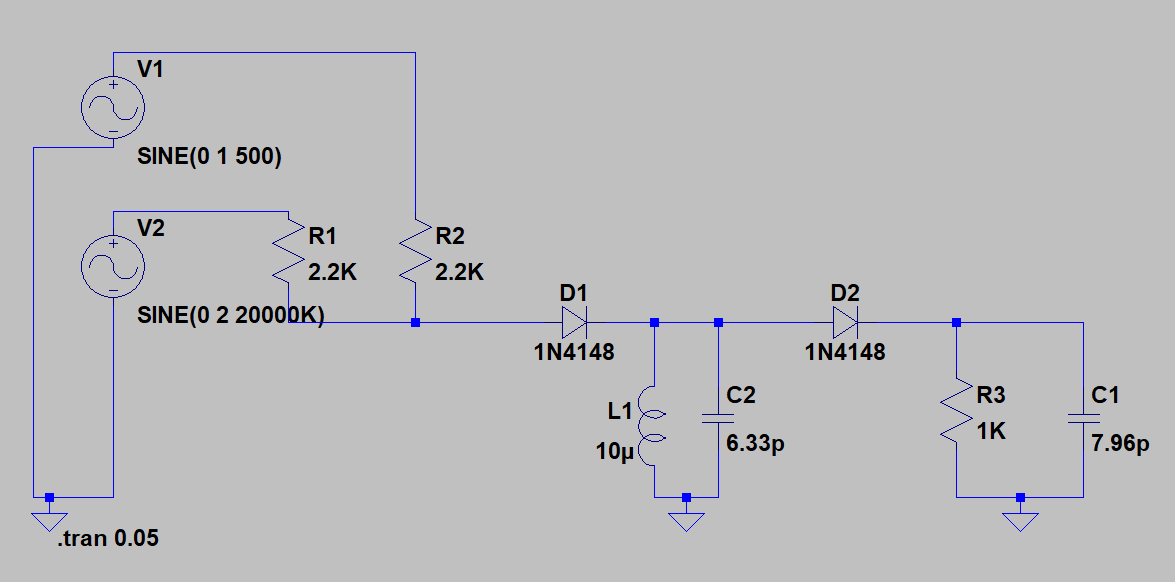
\includegraphics[width=0.7\textwidth]{images/circuit_1.png}
		\caption{LTSpice circuit used for this experiment}
	\end{figure}

	The values for the capacitors for the modulator and the demodulator circuits were calculated according to the rules as laid out in the theoretical background section of this document.

	$C2$ was calculated according to the equation given as 
	\begin{equation}
		f =  \frac{1}{2\pi\sqrt{LC}} 
		\label{eqn:capacitor_modulator_circuit}
	\end{equation}

	Where $L$ is given as $L = 10\times10^{-6}H$ and the frequency is given as $f= 20\times 10^6 $Hz. Substituting this into equation \ref{eqn:capacitor_modulator_circuit} we get that the capacitor needed for the modulator circuit is
	\[
		\begin{array}{rcl}
			f & = & \frac{1}{2\pi\sqrt{LC_2}} \\
			2\pi f \sqrt{L} & = & \frac{1}{\sqrt{C_2}} \\
			\sqrt{C_2} & = & \frac{1}{2\pi f \sqrt{L}} \\
			C_2 & = & \left(\frac{1}{2\pi f \sqrt{L}}\right)^2 \\
			& = & \left(\frac{1}{2\pi(20\times 10^6)\sqrt{10\times 10^{-6}}}\right)^2 \\
			& = & 6.33257 \times 10^{-12} \\
			& \approx & 6.33 pF 
		\end{array}
	\]

	$C_1$ was calculated using equation \ref{eqn:time_const_demodulator_circuit}. Taking $RC$ to be given as $\frac{1}{\omega_c}$, where $\omega_c$ is the angular frequency of the carrier signal given as $125.66 \times 10^6 $. Using these values we find that $C_1$ is given as

	\[
		\begin{array}{rcl}
			RC_1 & = & \frac{1}{\omega_c} \\
			C_1 & = & \frac{1}{\omega_c R} \\
			& = & \frac{1}{2\pi (20\times 10^6)(1000)} \\
			& = & 7.95775 \times 10^{-12} \\
			& \approx & 7.96 pF
		\end{array}
	\]


% section experimental_method (end)

\section{Results} % (fold)
\label{sec:results}
	\begin{figure}[H]
		\centering
		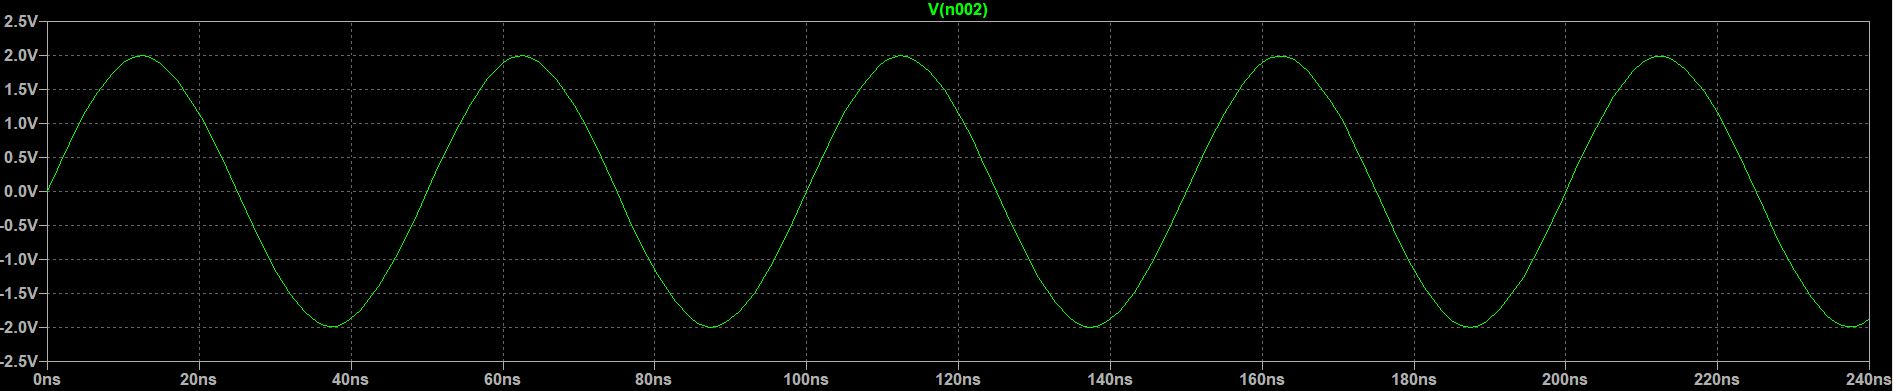
\includegraphics[width=\textwidth]{images/carrier.JPG}
		\caption{20 MHz Carrier signal}
		\label{fig:carrier}
	\end{figure}

	\begin{figure}[H]
		\centering
		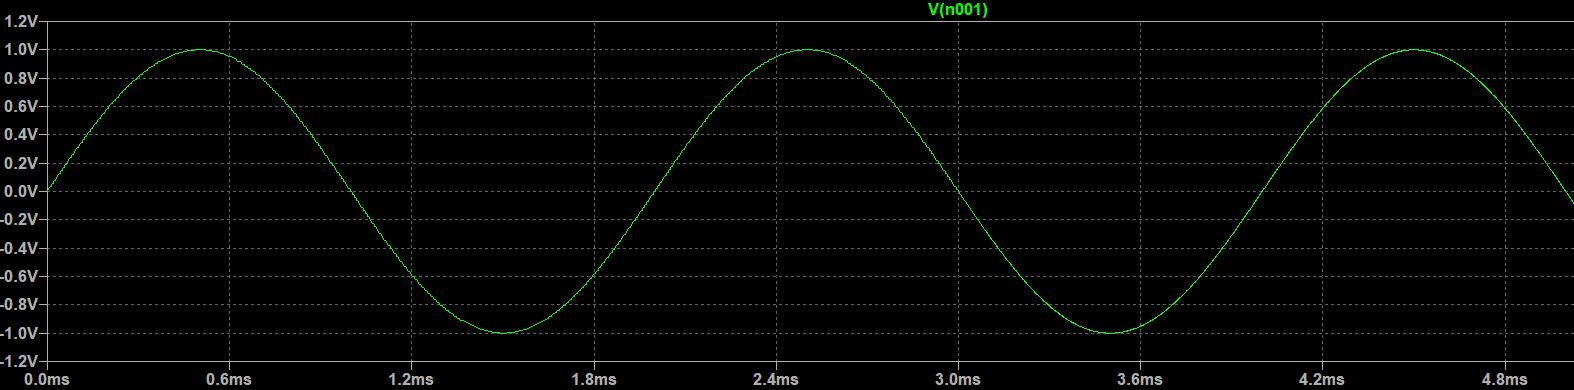
\includegraphics[width=\textwidth]{images/modulating.JPG}
		\caption{500 Hz input signal}
		\label{fig:modulating}
	\end{figure}

	\begin{figure}[H]
		\centering
		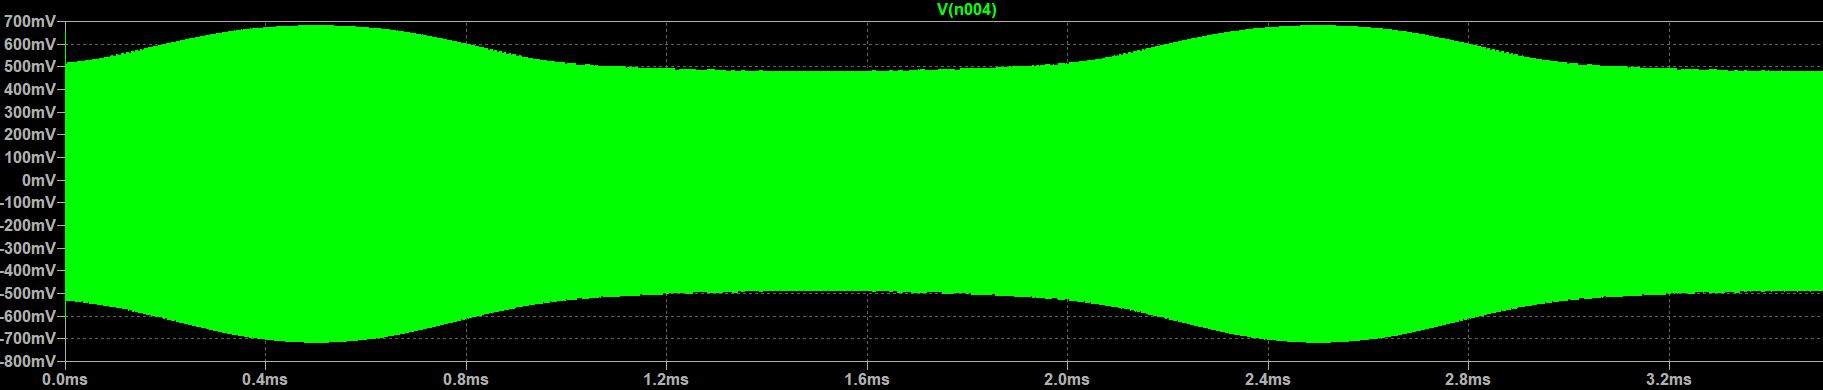
\includegraphics[width=\textwidth]{images/output_modulated.JPG}
		\caption{Modulator output}
		\label{fig:output_modulated}
	\end{figure}

	\begin{figure}[H]
		\centering
		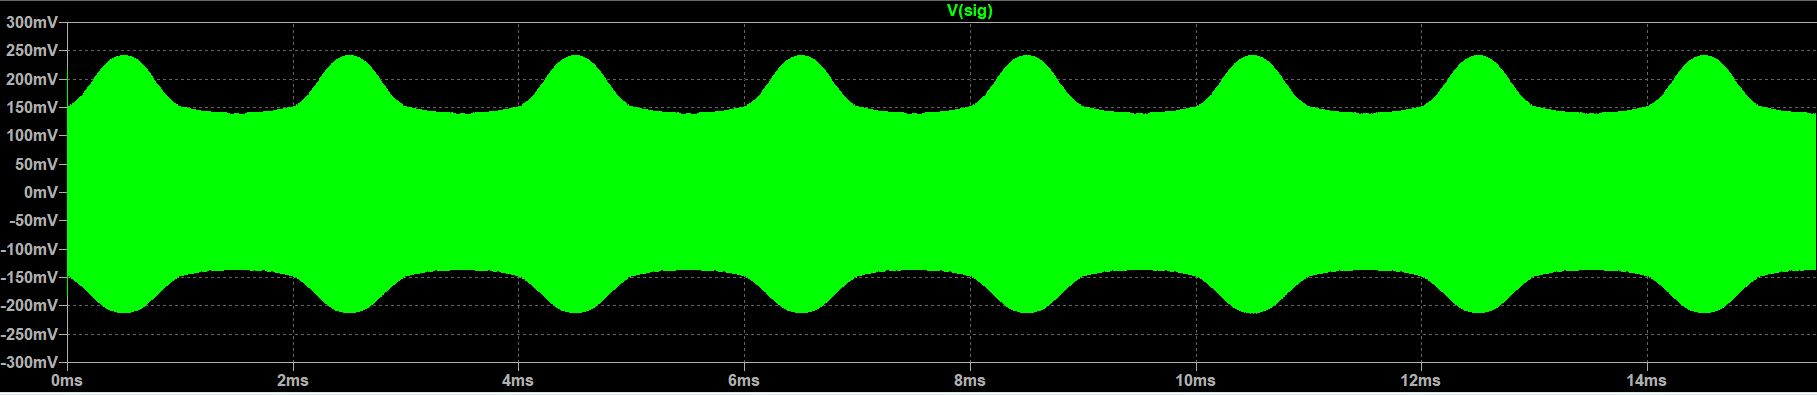
\includegraphics[width=\textwidth]{images/output_demodulated.JPG}
		\caption{Demodulated output}
		\label{fig:output_demodulated}
	\end{figure}
% section results (end)

\section{Discussion} % (fold)
\label{sec:discussion}
	In this practical, we have chosen the carrier wave with a frequency of 20 MHz, and an amplitude of $2V$. In order to simulate audio input, we simply chose a signal generator which generates a 500 Hz sine wave at an amplitude of $1V$. These two signals can be seen in Figure \ref{fig:carrier} and Figure \ref{fig:modulating}. What we expect at the modulated output of the circuit, theoretically, is to have a 20 MHz signal that has the envelope of the 500 Hz sine wave input. From Figure \ref{fig:output_modulated} we can see that this is indeed the case.

	The signal looks ``solid'' due to the large difference between the frequencies of the carrier and modulating waves. It is instructive to note that, due to the constraints of the practical, we had to choose a carrier signal that would require the capacitor $C_2$ in the circuit to have a value of $3pF \le C_2 \le 40pF$. Now, since the modulating signal is 500 Hz, we expect the envelope of the carrier signal to have a period once every 2$ms$. By inspecting the voltage values of Figure \ref{fig:output_modulated}, we see that the modulated signal at 0$ms$ is approximately $514mV$. The value of the modulated signal at $2ms$ is also $514mV$. Therefore we can conclude that the envelope of the carrier signal is indeed correct.

	In Figure \ref{fig:output_demodulated} shows the demodulated output of the circuit. By visual inspection, it can still be seen that the signal has an envelope of 500 Hz, as it is periodic, and repeats every $2ms$. From the envelope, however, it appears that the bottom half of the 500 Hz modulating signal is somewhat distorted.\linebreak

	There is quite a difference in the amplitudes of the modulated and demodulated signals. We would expect, mathematically, that the two signals should have a maximum amplitude of $2V$, as the carrier and modulating signals peak at $2V$ and $1V$ respectively. However, the modulated output signal has a maximum output of around $700mV$, while the demodulated output signal has a maximum signal of approximately $250mV$. One reason for this reduction in voltage is due the modulating and demodulating process. The modulation process has an LC circuit, whose impedance acts to attenuate the voltage of the signal. A voltage drop across the diodes in the circuit also serve to reduce the maximum amplitude of the output voltage. It is clear that this signal will have to be at some stage during the encoding process, so that higher level signals can be obtained.
% section discussion (end)

\section{Conclusion} % (fold)
\label{sec:conclusion}
	
% section conclusion (end)

\begin{thebibliography}{500}

	\bibitem{lamport94}
	  Donald A. Neamen,
	  \textit{Microelectronics: Circuit Analysis and Design}

	\bibitem{Detector}
	Phil Frost
	\textit{RC time constant and diode detector}
	\texttt{https://electronics.stackexchange.com/questions/100518/\\rc-time-constant-and-diode-detector}

\end{thebibliography}

\end{document}